\section{Auswertung}
\label{sec:Auswertung}
\subsection{Nullrate}
\label{sec:Nullrate}
Vor der eigentlichen Messung wird die Nullrate bestimmt. Um den statistischen Fehler möglichst gering zu halten,
wird für eine Zeit von $t=500\,\unit{\second}$ gemessen. Bei dieser Messzeit ergibt sich eine Zählrate von
$N=150$. Die Nullrate bestimmt sich dadurch zu $N_{\symup{u}}=3$ pro $10\,\unit{\second}$ oder zu
$N_{\symup{u}}=9$ pro $30\,\unit{\second}$. Im Folgenden wird die Nullrate immer von den Messwerten abgezogen.

\section{Halbwertszeit von Vanadium}
\label{sec:Vanadium}
Um die Halbwertszeit von Vanadium zu bestimmen, wird die mittlere Zählrate halblogarithmisch gegen die Zeit
in \autoref{fig:vanadium} aufgetragen. Die gemessen Werte samt des $\sqrt{N}$-Fehlers sind in \autoref{tab:vanadium}
zu finden.
\begin{table}
  \centering
  \begin{tabular}{c c}
    \toprule
    Messzeit $t/\unit{\second}$ & Zählrate $N$\\
    \midrule
     30 & 131 $\pm$ 11 \\
     60 & 116 $\pm$ 11 \\
     90 & 122 $\pm$ 11 \\
    120 &  88 $\pm$  9 \\
    150 &  91 $\pm$ 10 \\
    180 &  72 $\pm$  1 \\
    210 &  81 $\pm$  8 \\
    240 &  63 $\pm$  9 \\
    270 &  58 $\pm$  8 \\
    300 &  40 $\pm$  8 \\
    330 &  57 $\pm$  6 \\
    360 &  36 $\pm$  8 \\
    390 &  40 $\pm$  6 \\
    420 &  40 $\pm$  6 \\
    450 &  49 $\pm$  6 \\
    \bottomrule
  \end{tabular}
  \begin{tabular}{c c}
    \toprule
    Messzeit $t/\unit{\second}$ & Zählrate $N$\\
    \midrule
    480 &  28 $\pm$ 7 \\
    510 &  19 $\pm$ 5 \\
    540 &  29 $\pm$ 4 \\
    570 &  28 $\pm$ 5 \\
    600 &  19 $\pm$ 5 \\
    630 &   9 $\pm$ 4 \\
    660 &  22 $\pm$ 3 \\
    690 &  13 $\pm$ 5 \\
    720 &  12 $\pm$ 4 \\
    750 &  12 $\pm$ 3 \\
    780 &  12 $\pm$ 3 \\
    810 &  12 $\pm$ 3 \\
    840 &   6 $\pm$ 2 \\
    870 &   9 $\pm$ 3 \\
    900 &   5 $\pm$ 2 \\
    \bottomrule
  \end{tabular}
  \caption{Messwerte der Zählrate für Vanadium.}
  \label{tab:vanadium}
\end{table}
Der Fehler für die gemittelte Zählrate ergibt sich durch die Gaußsche Fehlerforpflanzung, die durch
\begin{align*}
  \Delta\bar{N} = \frac{1}{t}\cdot\Delta N
\end{align*}
gegeben ist. Mit Hilfe von \autoref{eqn:Zerfallsgesetz} lässt sich in halblogarithmischer Darstellung die
Gleichung
\begin{align*}
  N(t) = -\lambda t + \ln{N_{\symup{0}}}
\end{align*}
aufstellen. Mit Scipy lässt sich nun eine lineare Regression mit den Ergebnissen
\begin{align*}
  \lambda_{\symup{Vanadium}} &= (6,40 \pm 0,28)*10^{-3} \frac{1}{\unit{\second}} \\
  \ln{N_{\symup{0, Vanadium}}} &= 0,49 \pm 0,15 \\
  \Rightarrow N_{\symup{0, Vanadium}} &= 1,63 \pm 0,24 \\
\end{align*}
durchführen. Aus \autoref{eqn:T} ergibt sich dann für die Halbwertszeit von Vanadium
\begin{align*}
  T_{\symup{Vanadium}} = (108 \pm 5)\,\unit{\second}
\end{align*}

\begin{figure}
  \centering
  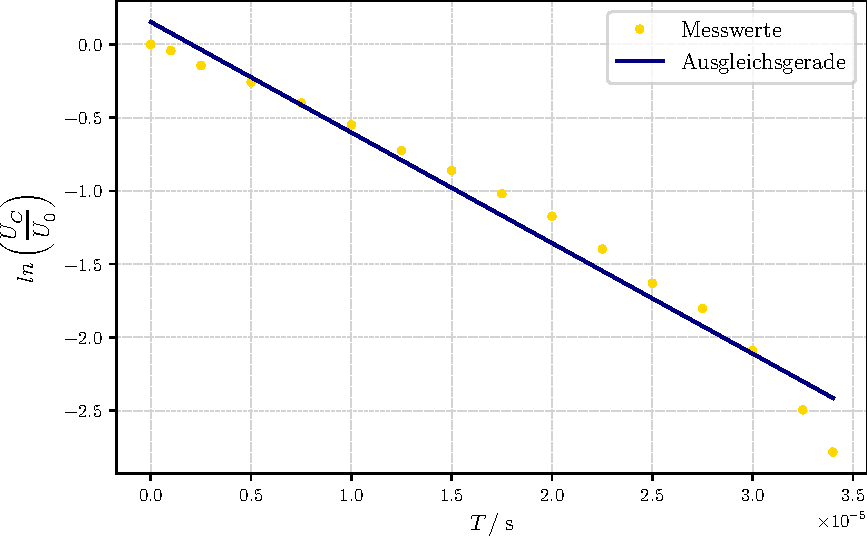
\includegraphics{plot1.pdf}
  \caption{Plot.}
  \label{fig:vanadium}
\end{figure}